\documentclass[a4paper, 11pt]{article}
\usepackage{comment} % enables the use of multi-line comments (\ifx \fi)
\usepackage{lipsum} %This package just generates Lorem Ipsum filler text.
\usepackage{fullpage} % changes the margin
\usepackage[a4paper, total={7in, 10in}]{geometry}
\usepackage[fleqn]{amsmath}
\usepackage{amssymb,amsthm}  % assumes amsmath package installed
\newtheorem{theorem}{Theorem}
\newtheorem{corollary}{Corollary}
\usepackage{graphicx}
\usepackage{tikz}
\usetikzlibrary{arrows}
\usepackage{verbatim}
\usepackage{pdfpages}
\usepackage[numbered]{mcode}
\usepackage{float}
\usepackage{tikz}
    \usetikzlibrary{shapes,arrows}
    \usetikzlibrary{arrows,calc,positioning}

    \tikzset{
        block/.style = {draw, rectangle,
            minimum height=1cm,
            minimum width=1.5cm},
        input/.style = {coordinate,node distance=1cm},
        output/.style = {coordinate,node distance=4cm},
        arrow/.style={draw, -latex,node distance=2cm},
        pinstyle/.style = {pin edge={latex-, black,node distance=2cm}},
        sum/.style = {draw, circle, node distance=1cm},
    }
\usepackage{xcolor}
\usepackage{mdframed}
\usepackage[shortlabels]{enumitem}
\usepackage{indentfirst}
\usepackage{hyperref}

\renewcommand{\thesubsection}{\thesection.\alph{subsection}}

\newenvironment{problem}[2][Problem]
    { \begin{mdframed}[backgroundcolor=gray!20] \textbf{#1 #2} \\}
    {  \end{mdframed}}

% Define solution environment
\newenvironment{solution}
    {\textit{Solution:}}
    {}

\renewcommand{\qed}{\quad\qedsymbol}
%%%%%%%%%%%%%%%%%%%%%%%%%%%%%%%%%%%%%%%%%%%%%%%%%%%%%%%%%%%%%%%%%%%%%%%%%%%%%%%%%%%%%%%%%%%%%%%%%%%%%%%%%%%%%%%%%%%%%%%%%%%%%%%%%%%%%%%%
\begin{document}
%Header-Make sure you update this information!!!!
\noindent
%%%%%%%%%%%%%%%%%%%%%%%%%%%%%%%%%%%%%%%%%%%%%%%%%%%%%%%%%%%%%%%%%%%%%%%%%%%%%%%%%%%%%%%%%%%%%%%%%%%%%%%%%%%%%%%%%%%%%%%%%%%%%%%%%%%%%%%%
\large\textbf{Jiawei Shan} \hfill \textbf{Homework - 13}   \\
Email: jwshan@ruc.edu.cn \hfill ID: 2019000151 \\
\normalsize Course: Linear Model   \hfill Term: Spring 2020\\
\noindent\rule{7in}{2.8pt}
%%%%%%%%%%%%%%%%%%%%%%%%%%%%%%%%%%%%%%%%%%%%%%%%%%%%%%%%%%%%%%%%%%%%%%%%%%%%%%%%%%%%%%%%%%%%%%%%%%%%%%%%%%%%%%%%%%%%%%%%%%%%%%%%%%%%%%%%
% Problem
%%%%%%%%%%%%%%%%%%%%%%%%%%%%%%%%%%%%%%%%%%%%%%%%%%%%%%%%%%%%%%%%%%%%%%%%%%%%%%%%%%%%%%%%%%%%%%%%%%%%%%%%%%%%%%%%%%%%%%%%%%%%%%%%%%%%%%%%
\begin{problem}{9.2.1}
  Consider the one-way layout. Show that when the model $y_{t r}=\mu+\varepsilon_{t r}$ is fitted, the residual sum of squares is $\sum_{r, t}\left(y_{t r}-\bar{y} . .\right)^{2}$ on $T R-1$ degrees of freedom, where $\bar{y}$.. is the overall average. Show that
  \[
  \sum_{r, t}\left(y_{t r}-\bar{y}_{. .}\right)^{2}=\sum_{r, t}\left(y_{t r}-\bar{y}_{t .}\right)^{2}+\sum_{r, t}\left(\bar{y}_{t .}-\bar{y}_{. .}\right)^{2}
  \]
  and hence verify the contents of Table 9.2.\\
 How would you form a confidence interval for $\beta_{1}-\beta_{2} ?$
\end{problem}
\begin{solution}
...
\end{solution}

\noindent\rule{7in}{2.8pt}

%%%%%%%%%%%%%%%%%%%%%%%%%%%%%%%%%%%%%%%%%%%%%%%%%%%%%%%%%%%%%%%%%%%%%%%%%%%%%%%%%%%%%%%%%%%%%%%%%%%%%%%%%%%%%%%%%%%%%%%%%%%%%%%%%%%%%%%%
% Problem
%%%%%%%%%%%%%%%%%%%%%%%%%%%%%%%%%%%%%%%%%%%%%%%%%%%%%%%%%%%%%%%%%%%%%%%%%%%%%%%%%%%%%%%%%%%%%%%%%%%%%%%%%%%%%%%%%%%%%%%%%%%%%%%%%%%%%%%%
\begin{problem}{9.2.4}
Give the analysis of variance table for a two-way layout with replication, when the numbers of replicates in the $t$ th row and $p$ th column, $J_{t p},$ are unequal.
\end{problem}
\begin{solution}
...
\end{solution}

\noindent\rule{7in}{2.8pt}


%%%%%%%%%%%%%%%%%%%%%%%%%%%%%%%%%%%%%%%%%%%%%%%%%%%%%%%%%%%%%%%%%%%%%%%%%%%%%%%%%%%%%%%%%%%%%%%%%%%%%%%%%%%%%%%%%%%%%%%%%%%%%%%%%%%%%%%%
% Problem
%%%%%%%%%%%%%%%%%%%%%%%%%%%%%%%%%%%%%%%%%%%%%%%%%%%%%%%%%%%%%%%%%%%%%%%%%%%%%%%%%%%%%%%%%%%%%%%%%%%%%%%%%%%%%%%%%%%%%%%%%%%%%%%%%%%%%%%%
\begin{problem}{9.3.1}
Suppose that a $2^{2}$ factorial experiment is to be performed using eight units in four blocks of two units each. Show that the intercept, three block effects, and the main effects and interaction between the treatments can be estimated if the treatments are allocated to blocks as follows: $(1, a),(b, a b),(1, a b),(a, b) .$ Can they all still be estimated if an observation from the last block is lost?
\end{problem}
\begin{solution}
...
\end{solution}

\noindent\rule{7in}{2.8pt}

%%%%%%%%%%%%%%%%%%%%%%%%%%%%%%%%%%%%%%%%%%%%%%%%%%%%%%%%%%%%%%%%%%%%%%%%%%%%%%%%%%%%%%%%%%%%%%%%%%%%%%%%%%%%%%%%%%%%%%%%%%%%%%%%%%%%%%%%
% Problem
%%%%%%%%%%%%%%%%%%%%%%%%%%%%%%%%%%%%%%%%%%%%%%%%%%%%%%%%%%%%%%%%%%%%%%%%%%%%%%%%%%%%%%%%%%%%%%%%%%%%%%%%%%%%%%%%%%%%%%%%%%%%%%%%%%%%%%%%
\begin{problem}{9.3.2}
  Table 9.21 gives results from a completely randomized experiment in which five individuals were allocated at random to each of three diets.
  \begin{enumerate}[(a)]
    \item Calculate the group averages and variances, and hence obtain the analysis of variance of the final weights, unadjusted for initial weights. Give the standard errors for differences between averages for diet A and the other two diets.
    \item Use analysis of covariance to adjust for the initial weights. Give the new analysis of variance table, and adjusted standard errors for the differences in (a). Comment.
  \end{enumerate}
\end{problem}
\begin{solution}
...
\end{solution}

\noindent\rule{7in}{2.8pt}

%%%%%%%%%%%%%%%%%%%%%%%%%%%%%%%%%%%%%%%%%%%%%%%%%%%%%%%%%%%%%%%%%%%%%%%%%%%%%%%%%%%%%%%%%%%%%%%%%%%%%%%%%%%%%%%%%%%%%%%%%%%%%%%%%%%%%%%%
% Problem
%%%%%%%%%%%%%%%%%%%%%%%%%%%%%%%%%%%%%%%%%%%%%%%%%%%%%%%%%%%%%%%%%%%%%%%%%%%%%%%%%%%%%%%%%%%%%%%%%%%%%%%%%%%%%%%%%%%%%%%%%%%%%%%%%%%%%%%%
\begin{problem}{9.3.3}
  Consider the calculation of a $95 \%$ confidence interval for the speed that gives the maximum efficiency for the field concrete mixer of Example 9.12.
  \begin{enumerate}[(a)]
    \item  Use the delta method to show that
    $$
    \operatorname{var}\left(\frac{\widehat{\gamma}_{1}}{\widehat{\gamma}_{2}}\right) \doteq \frac{\gamma_{1}^{2}}{\gamma_{2}^{2}}\left(\frac{\operatorname{var}(\widehat{\gamma_{1}})}{\gamma_{1}^{2}}+\frac{\operatorname{var}(\widehat{\gamma_{2}})}{\gamma_{2}^{2}}\right)
    $$
    Use this to show that $\widehat{\gamma}_{1} / \widehat{\gamma}_{2}$ has standard error $1.595,$ and hence give an approximate $95 \%$ confidence interval for $10-4 \gamma_{1} / \gamma_{2}$.

    \item If $\psi=-\gamma_{1} / \gamma_{2},$ show that the distribution of $\widehat{\gamma}_{2} \psi+\widehat{\gamma}_{1}$ is normal with mean zero and variance $\sigma^{2}\left(\psi^{2} v_{22}+v_{11}\right),$ where $v_{11}$ and $v_{22}$ are the diagonal elements of the matrix $\left(X^{\mathrm{T}} X\right)^{-1}$
    that correspond to $\gamma_{1}$ and $\gamma_{2} .$ Deduce that as $(\widehat{\gamma_{2}} \psi+\widehat{\gamma_{1}})^{2} /\left\{s^{2}\left(\psi^{2} v_{22}+v_{11}\right)\right\}$
    has an $F_{1, v}$ distribution, an exact confidence region for $\psi$ is the set of values such that $(\widehat{\gamma_{2}} \psi+\widehat{\gamma_{1}})^{2} /\left\{s^{2}\left(\psi^{2} v_{22}+v_{11}\right)\right\} \leq F_{1, v}(1-\alpha)$.\\
    A $95 \%$ confidence set for $10+4 \psi$ based on the calculations in Example 9.12 is $(-\infty, 9.15),(38.03, \infty) .$ On the same graph, plot this confidence set, the average efficiencies for the different speeds and the fitted efficiency from Example 9.12 against speed. Do you find the exact confidence set surprising?

    \item Use part (b) to calculate the exact coverage of your delta method confidence interval.
  \end{enumerate}

\end{problem}
\begin{solution}
...
\end{solution}

\noindent\rule{7in}{2.8pt}

%%%%%%%%%%%%%%%%%%%%%%%%%%%%%%%%%%%%%%%%%%%%%%%%%%%%%%%%%%%%%%%%%%%%%%%%%%%%%%%%%%%%%%%%%%%%%%%%%%%%%%%%%%%%%%%%%%%%%%%%%%%%%%%%%%%%%%%%
% Problem
%%%%%%%%%%%%%%%%%%%%%%%%%%%%%%%%%%%%%%%%%%%%%%%%%%%%%%%%%%%%%%%%%%%%%%%%%%%%%%%%%%%%%%%%%%%%%%%%%%%%%%%%%%%%%%%%%%%%%%%%%%%%%%%%%%%%%%%%
\begin{problem}{9.6.1}
  Example 9.6 is a $t w o-w a y$ layout with replication, in which the $j$ th replicate in row $r$ and column $c$ is
  \[
  y_{r c j}=\mu+\alpha_{r}+\beta_{c}+\gamma_{r c}+\varepsilon_{r c j}, \quad r=1, \ldots, R, \quad c=1, \ldots, C, \quad j=1, \ldots, k
  \]
  The $\alpha_{r}$ and $\beta_{c}$ represent the main effects of rows and columns; the $\gamma_{r c}$ are row $\times$ column interactions; and $\varepsilon_{r c j} \stackrel{\text { iid }}{\sim} N\left(0, \sigma^{2}\right)$.
  \begin{enumerate}[(a)]
    \item (a) Explain why an external estimate of $\sigma^{2}$ is needed if the $\gamma_{r c}$ are known not to be constant, and $k=1$.

    \item A first step in the analysis of such data is to calculate the cell mean and sums of squares $\bar{y}_{r c .}$ and $\sum_{j}\left(y_{r c j}-\bar{y}_{r c .}\right)^{2} .$ Show that the distribution of each cell sum of squares is $\sigma^{2} \chi_{k-1}^{2}$ and explain what you might expect to learn from a plot of $\log \sum_{j}\left(y_{r c j}-\bar{y}_{r c .}\right)^{2}$ against $\log y_{rc.}$.
    What does this plot show for the poisons data?

    \item The analysis of variance for this design is in Table $9.30 .$ Show that
    $$
    \mathrm{E}\left\{\sum_{r, c, j}\left(\bar{y}_{r . .}-\bar{y}_{. . .}\right)^{2}\right\}=(R-1) \sigma^{2}+k C \sum_{r}\left(\alpha_{r}-\bar{\alpha} .+\bar{\gamma}_{r .}-\bar{\gamma}_{..}\right)^{2}
    $$
    and write down $\mathrm{E}\left\{\sum_{r, c, j}\left(\bar{y}_{. c .}-\bar{y}_{. . .}\right)^{2}\right\} .$ Explain why these depend on the $\alpha_{r}$ and $\beta_{c}$ only through $\alpha_{r}-\bar{\alpha}$. and $\beta_{c}-\bar{\beta}_.$.

    $$\begin{array}{lcc}
    \multicolumn{1}{c}
    {}&\textbf{Table 9.30} &{} \\
    \hline {\text { Terms }} &\text { de of squares } & \text { Sum of } \\
    \hline \text { Rows } & R-1 & \sum_{r, c, j}\left(\bar{y}_{r \cdots}-\bar{y} \ldots\right)^{2} \\
    \text { Columns } & C-1 & \sum_{r, c, j}\left(\bar{y}_{\cdot c \cdot}-\bar{y}_{\ldots}\right)^{2} \\
    \text { Rows } \times \text { Columns } & (R-1)(C-1) & \sum_{r, c, j}\left(\bar{y}_{r c \cdot}-\bar{y}_{r . .}-\bar{y}_{. c .}+\bar{y}_{\ldots}\right)^{2} \\
    \hline \text { Residual } & R C(k-1) & \sum_{r, c, j}\left(y_{r c j}-\bar{y}_{r c .}\right)^{2} \\
    \hline
    \end{array}$$

    \item Show that
    $$\mathrm{E}\left\{\sum_{r, c, j}\left(\bar{y}_{r c .}-\bar{y}_{r . .}-\bar{y}_{.c .}+\bar{y}_{\ldots}\right)^{2}\right\}=(R-1)(C-1) \sigma^{2}+k \sum_{r c}\left(\gamma_{r c}-\bar{\gamma}_{r .}-\bar{\gamma}_{\cdot c}+\bar{\gamma}_{..}\right)^{2}$$
    Under what circumstances does this equal $(R-1)(C-1) \sigma^{2} ?$
  \end{enumerate}
\end{problem}
\begin{solution}
...
\end{solution}

\noindent\rule{7in}{2.8pt}

%%%%%%%%%%%%%%%%%%%%%%%%%%%%%%%%%%%%%%%%%%%%%%%%%%%%%%%%%%%%%%%%%%%%%%%%%%%%%%%%%%%%%%%%%%%%%%%%%%%%%%%%%%%%%%%%%%%%%%%%%%%%%%%%%%%%%%%%
% Problem
%%%%%%%%%%%%%%%%%%%%%%%%%%%%%%%%%%%%%%%%%%%%%%%%%%%%%%%%%%%%%%%%%%%%%%%%%%%%%%%%%%%%%%%%%%%%%%%%%%%%%%%%%%%%%%%%%%%%%%%%%%%%%%%%%%%%%%%%
\begin{problem}{9.6.2}
  Let $y_{g r}, g=1, \ldots, G, r=1, \ldots, R,$ be independent normal random variables with means $\mu_{g r}$ and common variance $\sigma^{2}$.
  \begin{enumerate}[(a)]
    \item  Assume the one-way analysis of variance model, namely that $\mu_{g r}=\mu_{g},$ so that the $y_{g r}$ are replicate measurements with the same mean, and find the sufficient statistics for the $\mu$ s and $\sigma^{2}$. Show that these are equivalent to
    $$
    \bar{y}_{1 .}, \ldots, \bar{y}_{G .}, \quad S S=\sum_{g=1}^{G} \sum_{r=1}^{R}\left(y_{g r}-\bar{y}_{g .}\right)^{2}
    $$
    where $\bar{y}_{g .}=R^{-1} \sum_{r=1}^{R} y_{g r} ;$ note that
    $$
    \sum_{r}\left(y_{g r}-\mu_{g}\right)^{2}=\sum_{r}\left(y_{g r}-\bar{y}_{g .}\right)^{2}+R\left(\bar{y}_{g .}-\mu_{g}\right)^{2}
    $$

    \item Prove that $S S$ is independent of the group means, and that it is proportional to a chi-squared random variable on $G(R-1)$ degrees of freedom.

    \item Let $\bar{y}_{\dots}=G^{-1} \sum_{g} \bar{y}_{g}$. denote the overall mean. If $\mu_{1}=\cdots=\mu_{G},$ show that the distribution of $S S_{G}=R \sum_{g=1}^{G^{8}}\left(y_{g} .-\bar{y} .\right)^{2}$ is proportional to a chi-squared distribution on $G-1$
    degrees of freedom. Hence find the distribution of $G(R-1) S S_{G} /(G-1) S^{2},$ when the means are equal.

    \item Samples of the same material are sent to four laboratories for chemical analysis as part of a study to determine whether laboratories give the same results. The results for laboratories A-D are:
    $$\begin{array}{llllll}
    \mathrm{A} & 58.7 & 61.4 & 60.9 & 59.1 & 58.2 \\
    \mathrm{B} & 62.7 & 64.5 & 63.1 & 59.2 & 60.3 \\
    \mathrm{C} & 55.9 & 56.1 & 57.3 & 55.2 & 58.1 \\
    \mathrm{D} & 60.7 & 60.3 & 60.9 & 61.4 & 62.3
    \end{array}$$
    Test the hypothesis that the means are different and comment.

  \end{enumerate}

\end{problem}
\begin{solution}
...
\end{solution}

\noindent\rule{7in}{2.8pt}

%%%%%%%%%%%%%%%%%%%%%%%%%%%%%%%%%%%%%%%%%%%%%%%%%%%%%%%%%%%%%%%%%%%%%%%%%%%%%%%%%%%%%%%%%%%%%%%%%%%%%%%%%%%%%%%%%%%%%%%%%%%%%%%%%%%%%%%%
% Problem
%%%%%%%%%%%%%%%%%%%%%%%%%%%%%%%%%%%%%%%%%%%%%%%%%%%%%%%%%%%%%%%%%%%%%%%%%%%%%%%%%%%%%%%%%%%%%%%%%%%%%%%%%%%%%%%%%%%%%%%%%%%%%%%%%%%%%%%%
\begin{problem}{Practicals 9.1}
See the last two pages.
\end{problem}
\begin{solution}
...
\end{solution}

\noindent\rule{7in}{2.8pt}


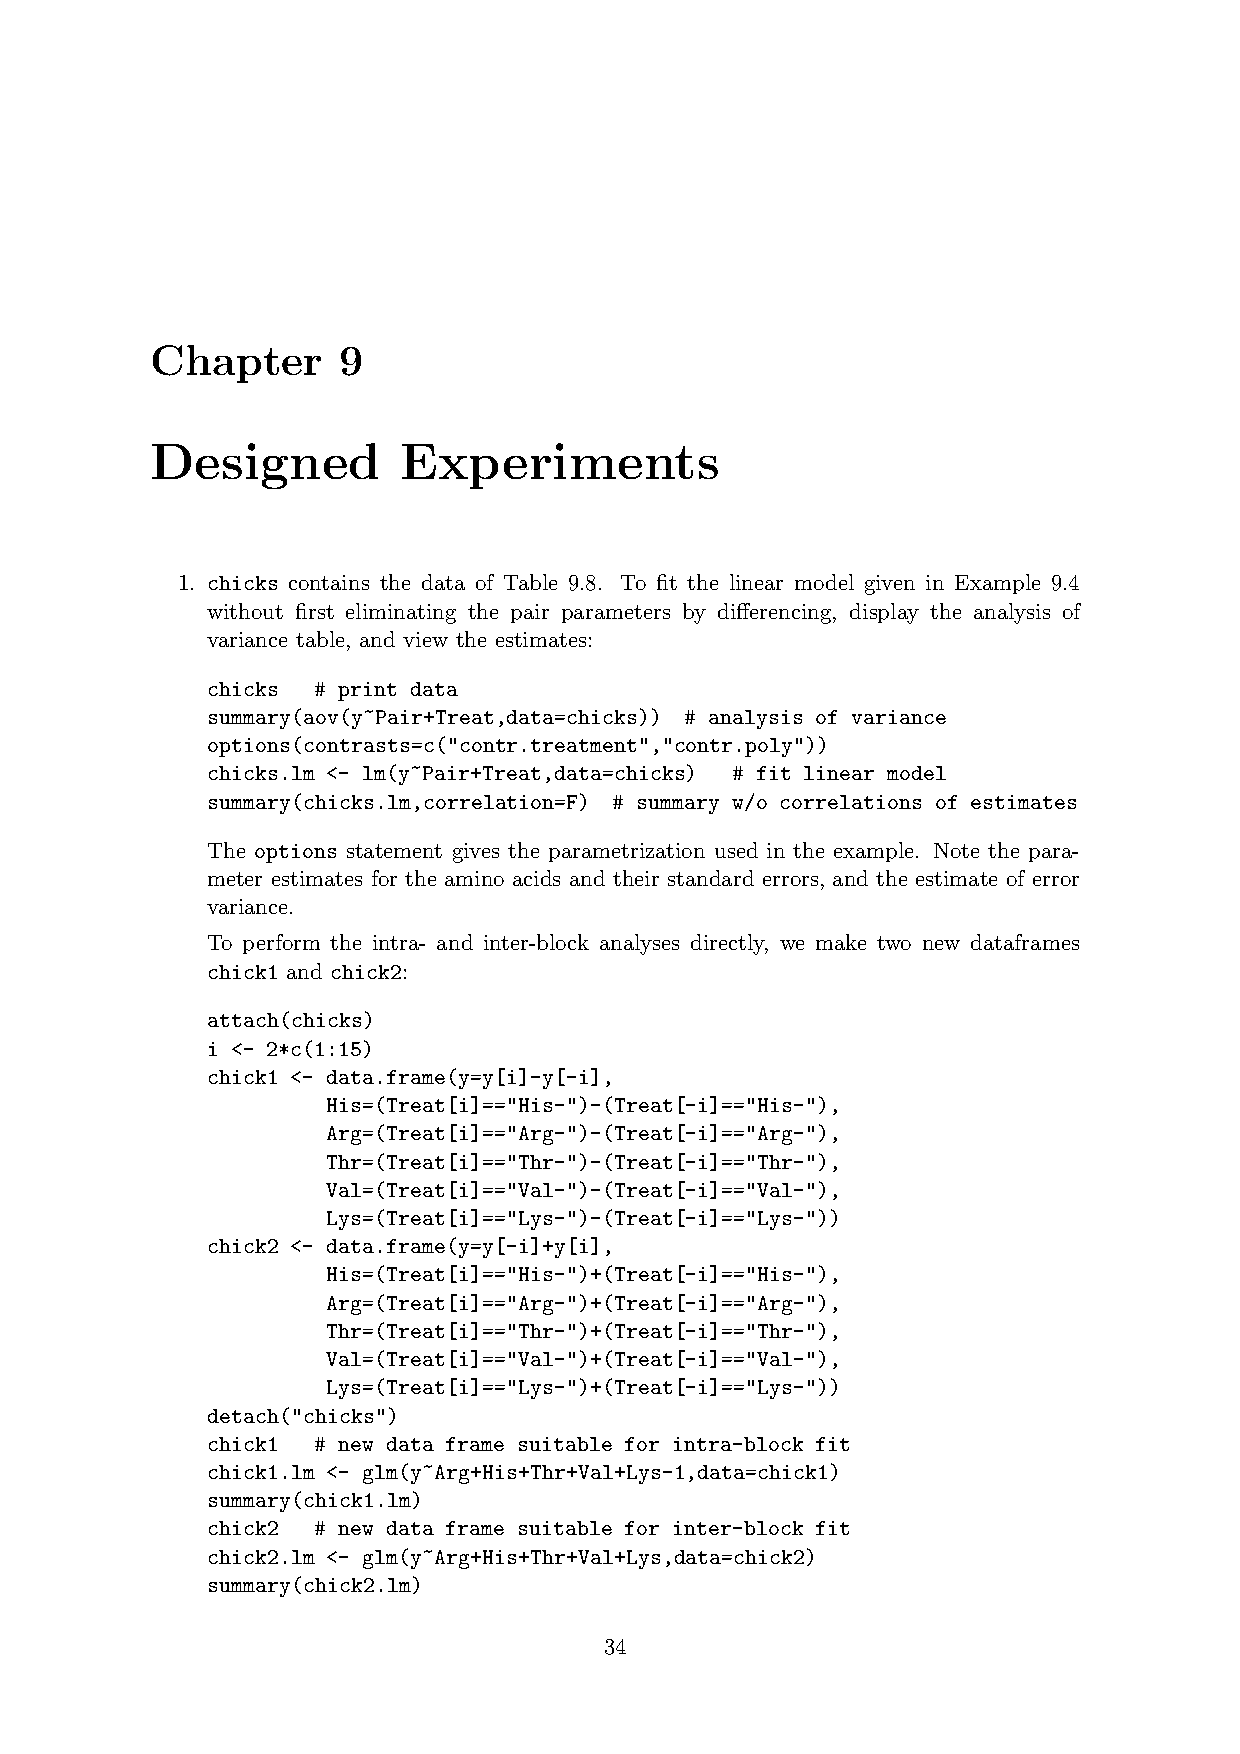
\includepdf[pages={1,2}]{week13_practical9_1.pdf}


% \begin{figure}[H]
%     \centering
%     \includegraphics[scale=0.25]{q2.png}
%     \caption{Plot showing $\hat{\phi}$ as a function of time.}
%     \label{fig_q2l}
% \end{figure}

% \begin{figure}[h]
%     \centering
%     \includegraphics[scale=0.6]{q2.png}
% \end{figure}

% \lstinputlisting{HW6Q2.m}
%%%%%%%%%%%%%%%%%%%%%%%%%%%%%%%%%%%%%%%%%%%%%%%%%%%%%%%%%%%%%%%%%%%%%%%%%
\end{document}
